\chapter{無線センサネットワーク}
\begin{large}
\begin{quote}
本節では,最初に多次元データ管理Multidimensional Indexing(MI)の分野における関連研究を挙げる.次に,Contents Delivery Network(CDN)におけるコンテンツの特徴を利用したレプリケーションを行った研究を挙げる.最後に,センサデータを多次元データとして扱った研究を挙げる.
\end{quote}
\end{large}
\clearpage

\section{はじめに}


\section{イベント検知アプリケーション}
\begin{figure}[htbp]
 \begin{center}
  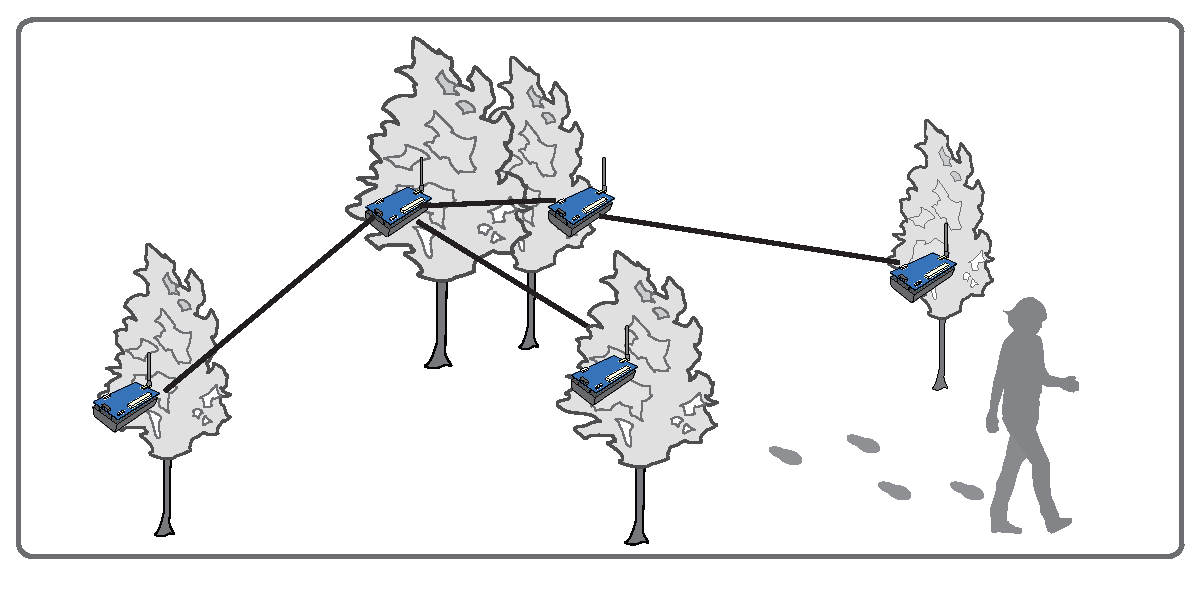
\includegraphics[width=100mm]{./images/event_detection.eps}
 \end{center}
 \caption{イベント検知アプリケーション}
 \label{fig:event_detection}
\end{figure}

\subsection{環境モニタリング}


\subsection{ターゲットトラッキング}


%\section{多次元データ管理}
%1990年代から,データベースの分野において,多次元のデータをどのように管理するべきかMultidimensional Indexing(MI)\cite{Gaede:1998:MAM:280277.280279}が議論されている.そして,地理学,ロボット工学,環境保護学などの様々な分野でこのMIは応用されている.1990年代のMIの中心はデータが集中管理されている環境を想定したアルゴリズムであり,VA\_File\cite{Weber:1998:QAP:645924.671192},Hilbert R-tree\cite{Kamel:1994:HRI:645920.673001},GHT\cite{Ratnasamy:2002:GGH:570738.570750}などがその代表である.2000年代からは,P2Pを用いた分散型のMIが主流となる.2000年代前半に提案されたChord\cite{Stoica:2001:CSP:383059.383071},CAN\cite{Ratnasamy:2001:SCN:383059.383072},SkipGraph\cite{Aspnes:2003:SG:644108.644170}が代表である.2000年代後半から現在にいたるまでにこれ以外の数多くのアルゴリズムが提案されているが,大半がこのいずれかのアルゴリズムの変形であって,大きなアルゴリズムの変化はない.
%
%センサデータが公衆化し,広域に管理される場合,2.2節で述べられているように,データの値以外のインデックスが付与される必要がある.よって,公衆広域センサデータを多次元データとして管理しなければならない.
%\begin{figure}[htbp]
% \begin{center}
%  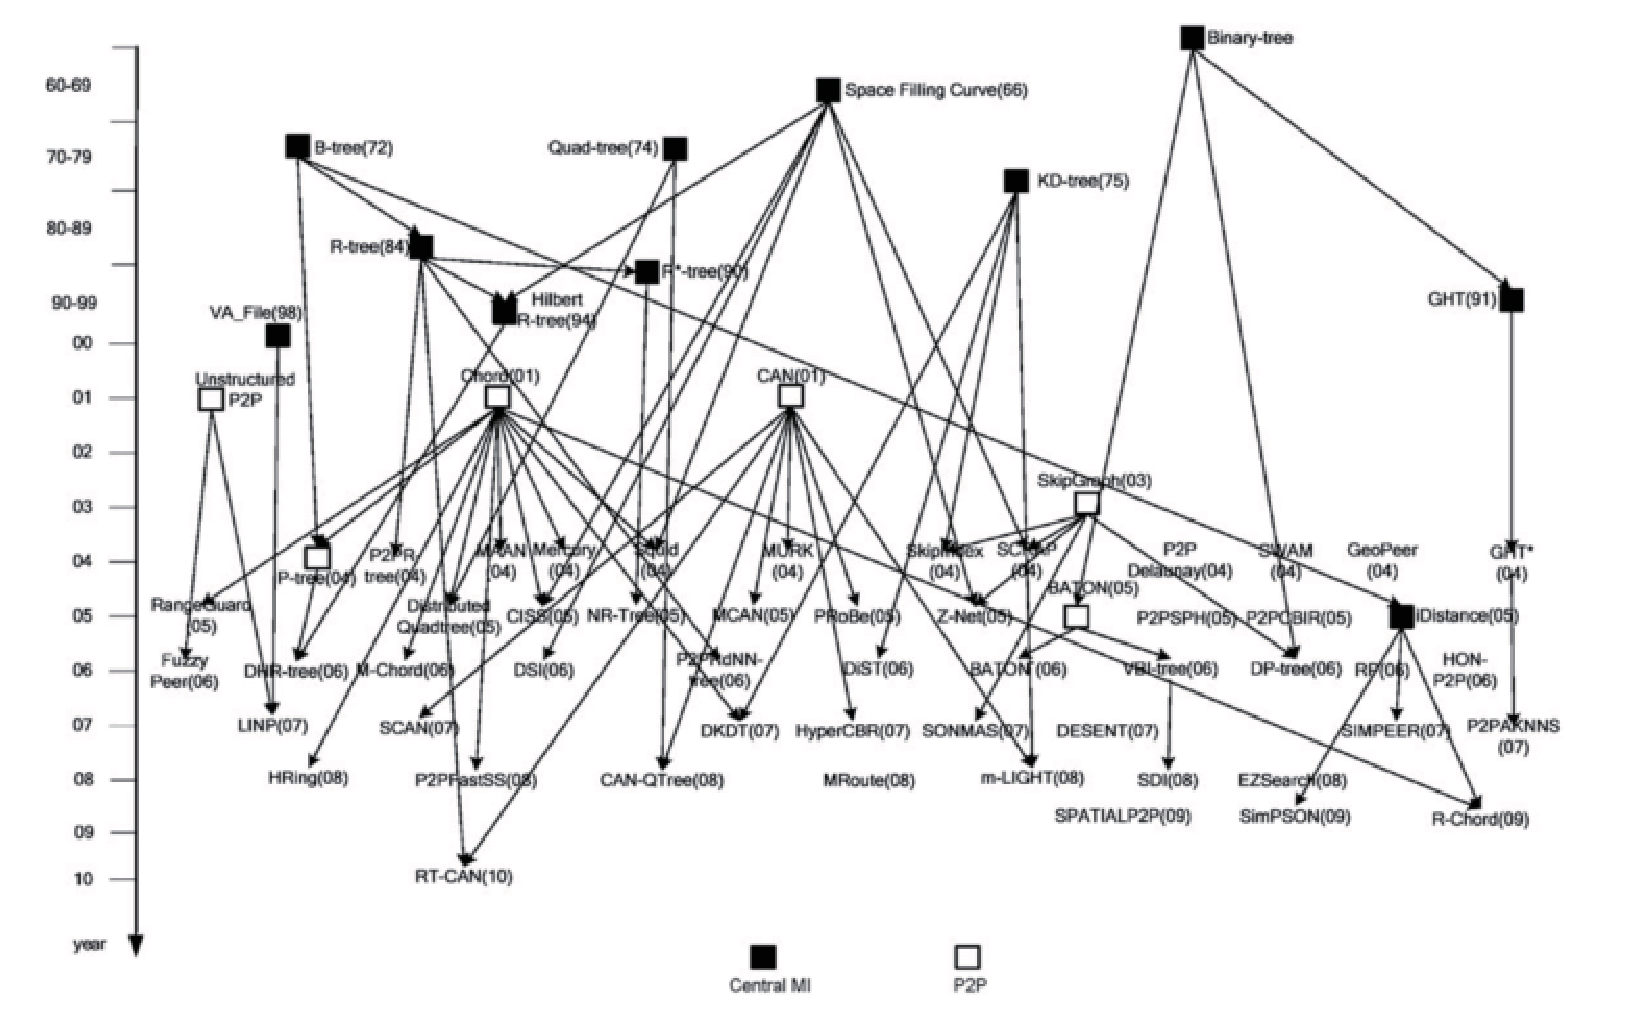
\includegraphics[width=130mm]{./images/MI_history.eps}
% \end{center}
% \caption{Multidimensional Indexingの歴史(参考:P2P-based multidimensional indexing methods. Journal of Systems and Software 2011\cite{Zhang:2011:PMI:2039458.2039840})}
% \label{fig:MI_history}
%\end{figure}
%
%
%
%\section{文書や音楽などのコンテンツの広域管理}
%この多次元データ管理は,Akamai\cite{Akamai}などに代表される,Contents Delivery Network(CDN)などで利用されている.CDNは世界中の数十,数百のデータセンターでP2Pネットワークを構築し,ユーザーに音楽や動画などを提供している.コンテンツには,サイズ,言語などの多次元のインデックスが付与されている.CDNは,コンテンツの特徴を抽出し,レプリケーション先を決定し,効率的なコンテンツの配送を実現している.Chaら\cite{Cha:2009:MAI:1526709.1526806}は,Flickr\cite{Flickr}のコンテンツがどのように伝播するのかの調査をしている.Scellatoら\cite{Scellato:2011:TGD:1963405.1963471}はtwitter\cite{twitter}やfacebook\cite{Facebook}などのSNSなどに載せられたコンテンツとその発言などのいち情報から,コンテンツの地域性を割り出し,レプリケーションを効率的に行う手法を提案している.Akamaiでは,トラフィックの状況などを公開しており,時間帯や地域による傾向を捉えることができる.関連研究ではコンテンツの言語から地域性を抽出し,対象地域のデータセンターに予めコンテンツをレプリケーションすることにより,効率化を実現している.この他にも,コンテンツや利用状況の特徴を抽出するために\cite{Tang:2012:MAA:2310257.2310450}\cite{Labovitz:2010:IIT:1851182.1851194}\cite{Maier:2009:DCR:1644893.1644904}\cite{Otto:2011:BME:2018436.2018450}などのインターネット計測の分野の研究結果も利用されている.
%
%\begin{figure}[htbp]
% \begin{center}
%  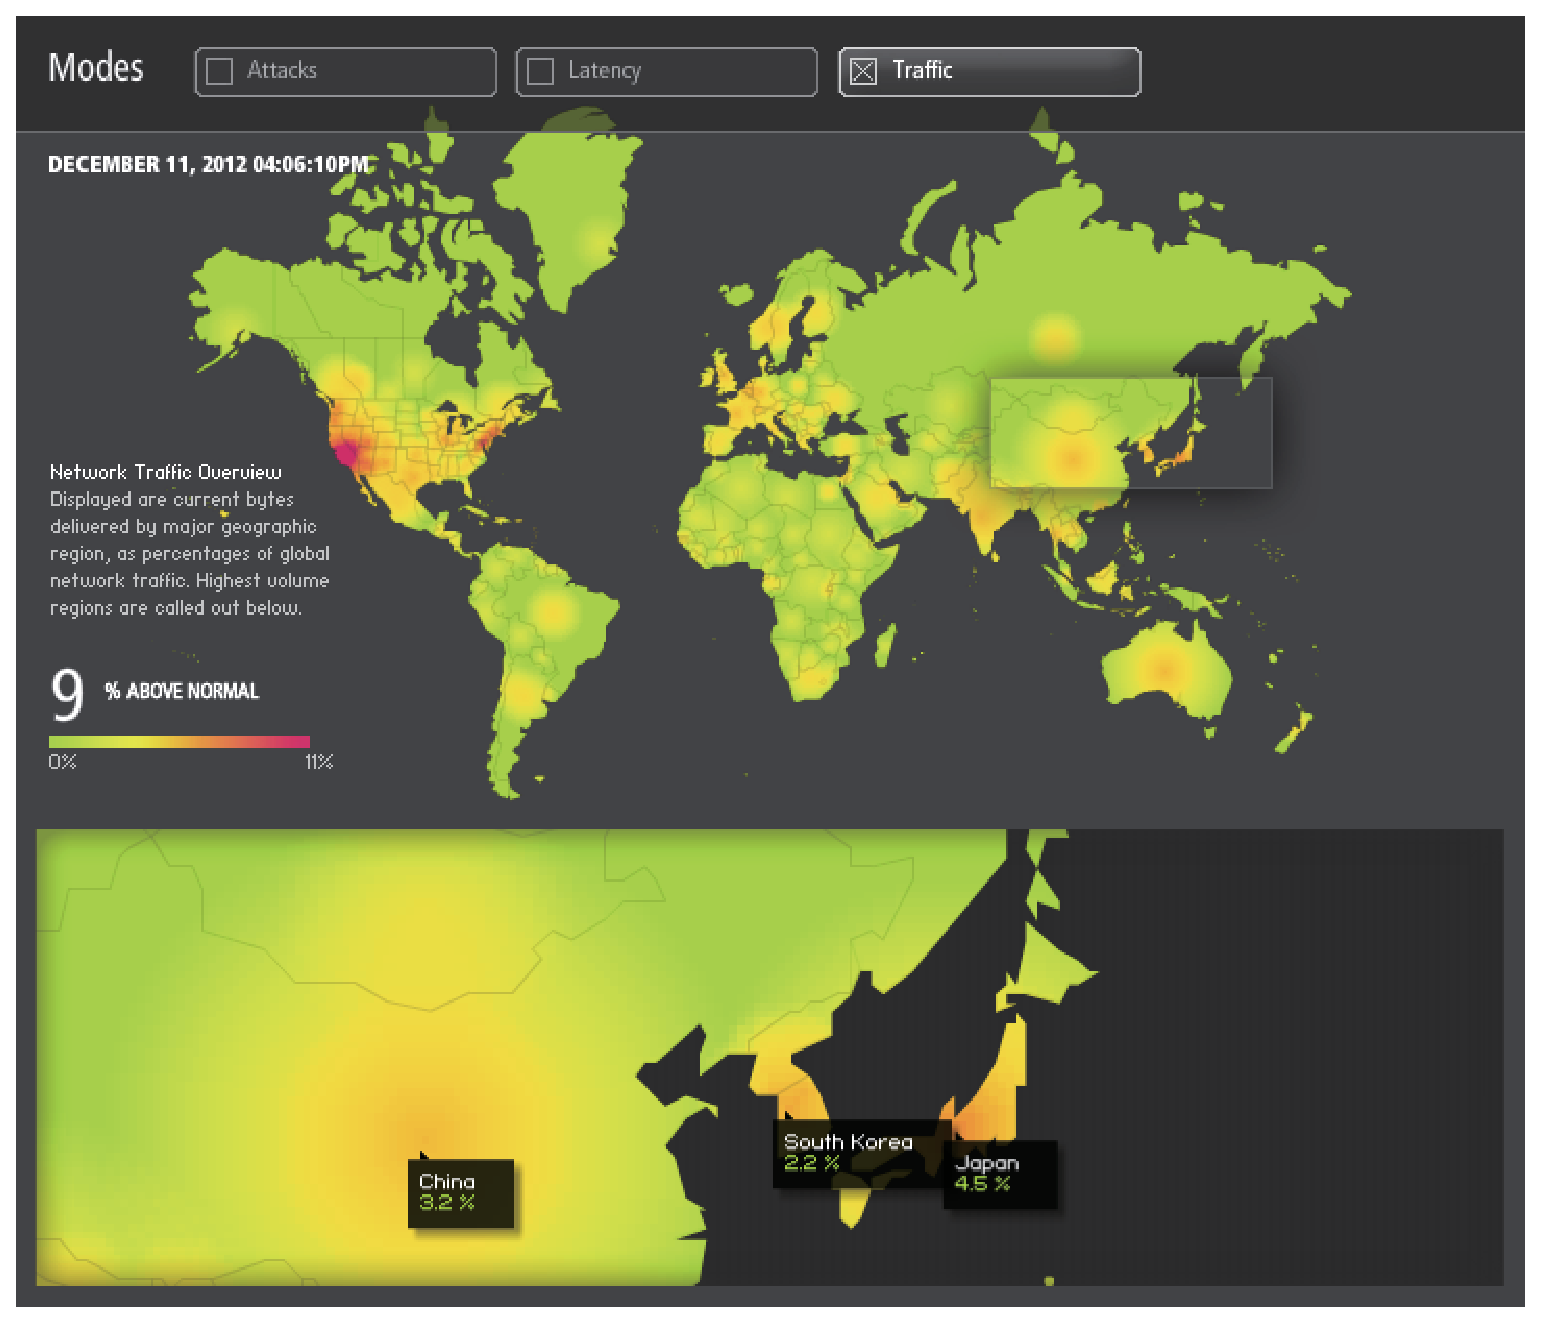
\includegraphics[width=100mm]{./images/akamai.eps}
% \end{center}
% \caption{Akamaiによるトラフィック情報の公開(参考:Akamai\cite{Akamai})}
% \label{fig:akamai}
%\end{figure}
%
%センサデータは2.3節で取り上げた,音楽や動画とは異なる時間的特殊性に加え,言語などから由来する地域性も存在しないため,コンテンツの特徴からレプリケーションの場所を決定するという手法を取ることができない.
%
%\section{DHTを用いた公衆センサデータ管理}
%広域センサデータを多次元データとして,MIのアルゴリズムを用いた研究にSynapse\cite{Terayama:2012:DSD:2370216.2370335}がある.この研究では,従来の,発せられたセンサデータを地理的に近い保存ストレージに保存するという手法では,イベントの発生による突発的な人口過密が発生した際に,特定のセンサデータ保存ストレージに対する保存,取得のクエリが集中すると主張している.そこで,センサデータの緯度,経度,センサタイプ,データの時間を空間充填曲線\cite{Lawder:2000:USC:646102.681186}図\ref{fig:zorder}を用いて1次元化する.空間充填曲線はLawderらが提案した,DHTアルゴリズムにおいて,多次元データを1次元化する手法で,これにより多次元データをハッシュ関数にかけることが可能になる.この手法はMIにおける基本的な手法であり,2009年にKantereらが提案したSPACIALP2P\cite{Kantere:2009:SIS:1495799.1496017}というMIアルゴリズムでも用いられている.このハッシュ化した値を元にDHTネットワークを構築することで,特定の保存ストレージに対するクエリの集中を防いでいる.
%
%しかし,Synapseではセンサデータの時間的特殊性が考慮されていないため,利用状況によっては,パフォーマンスが低下してしまう可能性がある.
%\begin{figure}[htbp]
% \begin{center}
%  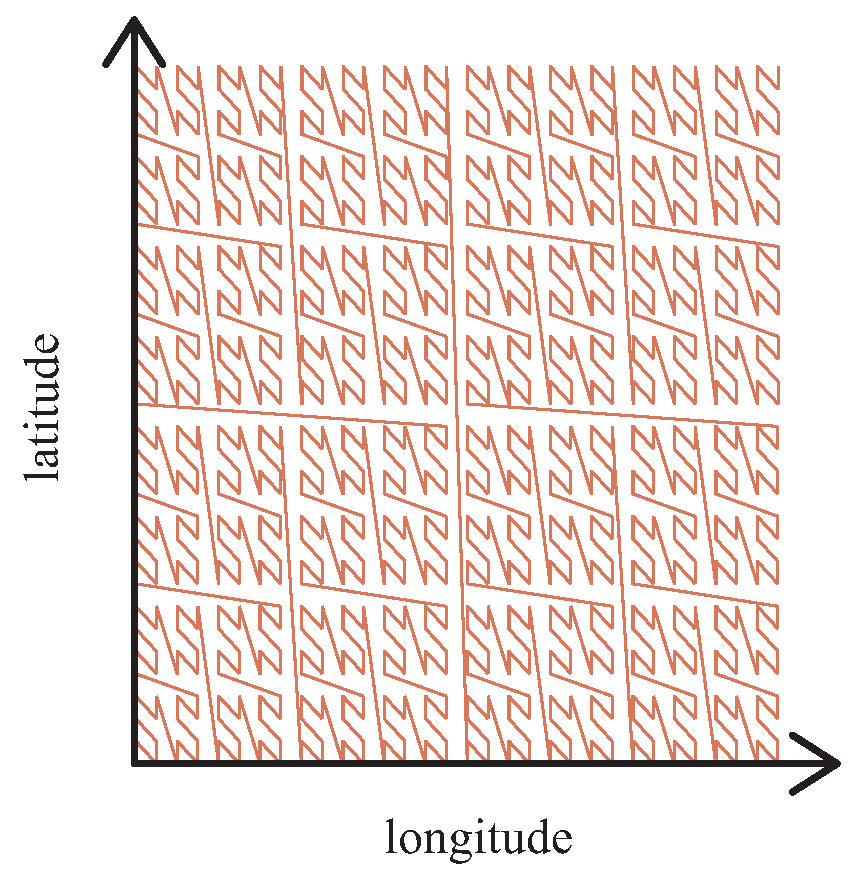
\includegraphics[height=100mm]{./images/zorder.eps}
% \end{center}
% \caption{空間充填曲線:Z-order}
% \label{fig:zorder}
%\end{figure}



\section{まとめ}
本章では,まず,公衆広域センサデータが多次元データであるということから,本研究の根幹を成す,Multidimensional Indexing(MI)という研究分野を紹介した.次に,Contents Delivery Network(CDN)という分散したデータセンターで多次元データを管理するネットワークという観点から捉え,センサデータにはCDNで扱われるような特殊性が存在しないことを述べた.最後に,公衆広域センサデータの分散管理手法を紹介し,センサデータの時間的特殊性が考慮されていないことに言及した.
